When formulating the test case search problem as a many-objective optimisation problem, the goal is to minimize all the individual distances from all the test targets in the class under test.

One of the most popular multi-objective algorithms for this problem is the Non-dominated Sorting Genetic Algorithm II (NSGA-II). This algorithm is based on three principles:

\begin{itemize}
    \item It uses elitism when evolving the population: the most fit individuals are carried over along the offsprings.
    \item It uses an explicit diversity-preserving mechanism, the Crowding distance.
    \item It emphasizes the non-dominated solutions, as its name suggests.
\end{itemize}

First of all, in the context of test cases, domination can be expressed by the following relation:
\begin{figure}[h]
    \centering
    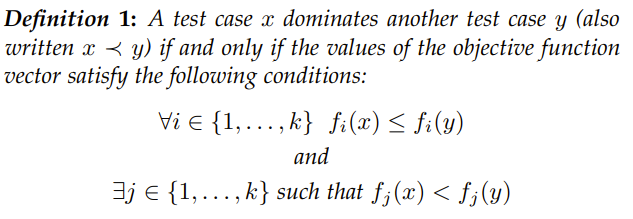
\includegraphics[scale=0.4]{./figures/test_Case_domination.PNG}
    \caption{Test case domination}
    \label{fig:test case domination}
\end{figure}


The NSGA-II algorithm works as follows:
\begin{itemize}
    \item Starting from an initial population of individuals Pt, generate an offspring population Qt of equal size and merge the two together, obtaining the population Rt.
    \item Perform non-dominated sorting of the individuals in Rt based on target indicatiors and classify them by fronts, i.e. the are sorted according to an ascending level of non-domination.  This ensures that the top Pareto-optimal individuals will survive to the next generation.
    \item If one of the fronts in the sorted sequence doesn't fit in terms of population size, crowding distance sorting is performed.
    \item Create the new population based on crowded tournament selection, then perform crossover and mutation. 
\end{itemize}


Figure 2.2 summarizes the main loop of the algorithm:
\begin{figure}[h]
    \centering
    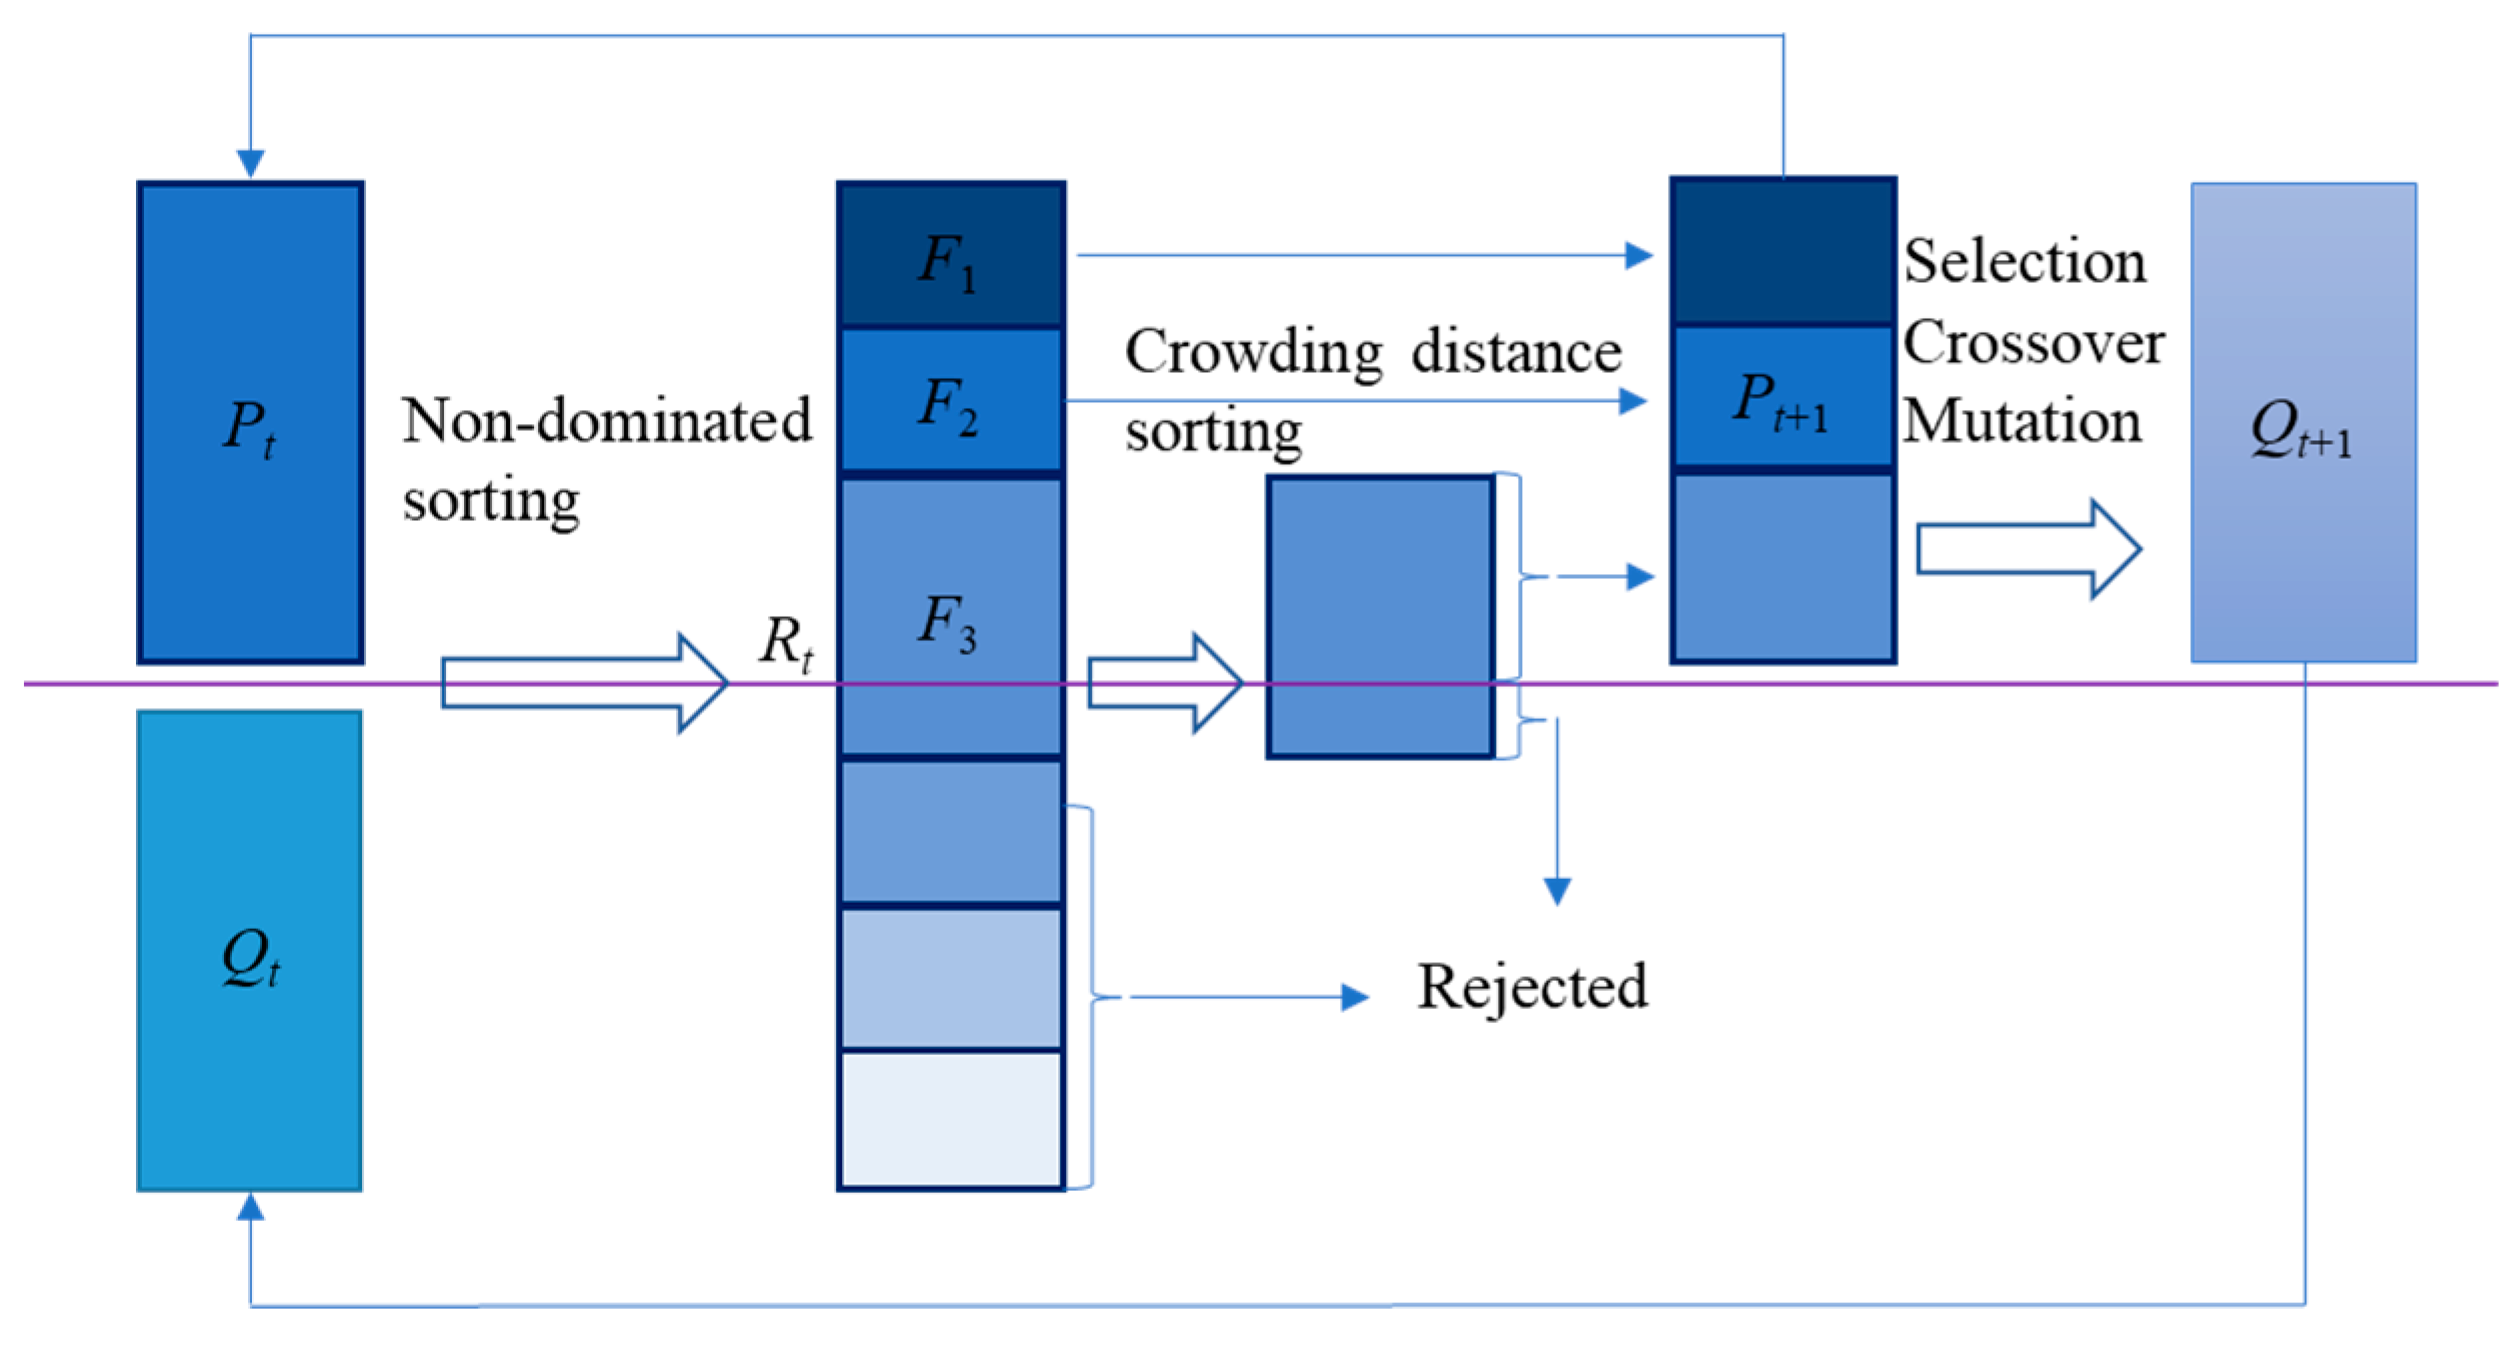
\includegraphics[scale=0.1]{./figures/nsga-ii.png}
    \caption{NSGA-II algorithm main loop}
    \label{fig:NSGA-II algorithm main loop}
\end{figure}


In the context of software enginnering, NSGA-II has been applied to problems such as software refactoring and test case prioritization,
with two or three objectives. If the number of objectives begins to grow, however, the performance of the algorithm doesn't scale up well \cite{article3}.
To overcome these limitation 


DynaMOSA, Dynamic Many-Objective Sorting Algorithm \cite{article1} is an approach that focuses on ..., and has been developed as an evolution of MOSA. This latter solution implements a many-objective GA to tackle test case generation and has three main features: 
\begin{itemize}
    \item instead of ranking candidates for selection based on their Pareto optimality, it uses a preference criterion. This criterion selects the test case with the lowest objective score for each uncovered target; these selected individuals are given a higher chance of survival, while other test cases are ranked with the traditional NSGA-II approach.
    \item The search is focused only on the uncovered coverage targets.
    \item All tests that satisfy one or more of the uncovered targets will be archived and used as the final test suite once the search ends.
\end{itemize}

In many-objective optimisation problems, candidate solutions are typically evaluated in terms of Pareto dominance and Pareto optimality.


DynaMOSA has been employed with Java classes.

Traditionally, with evolutionary search-based approaches, the algorithm is applied multiple times,  once for each coverage criterion; doing so may ... Ultimately, however, the effectiveness of the solution depends on the problem